\documentclass[11pt]{article}
\usepackage[utf8]{inputenc}
\usepackage[T1]{fontenc}
\usepackage[spanish]{babel}
\usepackage{amsmath,amssymb,amsthm,mathtools}
\usepackage{braket}
\usepackage{dsfont}
\usepackage{graphicx}
\usepackage{float}
\usepackage[margin=2.5cm]{geometry}
\usepackage{hyperref}
\hypersetup{hidelinks}
\emergencystretch=2em
\allowdisplaybreaks

\newcommand{\ii}{\mathrm{i}}
\newcommand{\Id}{\mathds{1}}

\title{Generaci\'on de estados entrelazados}
\author{Ricardo Del Rosal Gardu\~no \\ \small Doctorado en F\'isica, BUAP}
\date{Notas de doctorado}

\begin{document}
\maketitle
\tableofcontents
\bigskip

\section{Protocolo de entrelazamiento}

Se considera primero un estado coherente fon\'onico dentro de un bloque
polarit\'onico fijo. La pureza electr\'onica asociada con la bipartici\'on
electr\'on frente a fot\'on--fon\'on comienza en su valor m\'inimo,
$P_{\mathrm{el}}=1/2$, correspondiente a entrelazamiento m\'aximo para esta
bipartici\'on, y alcanza posteriormente el valor $P_{\mathrm{el}}=1$. En ese
instante el electr\'on se separa del subsistema fot\'on--fon\'on. La idea del
protocolo es localizar dicho estado separable, pues la evoluci\'on posterior
vuelve a conducirlo hacia estados entrelazados.

\begin{figure}[H]
  \centering
  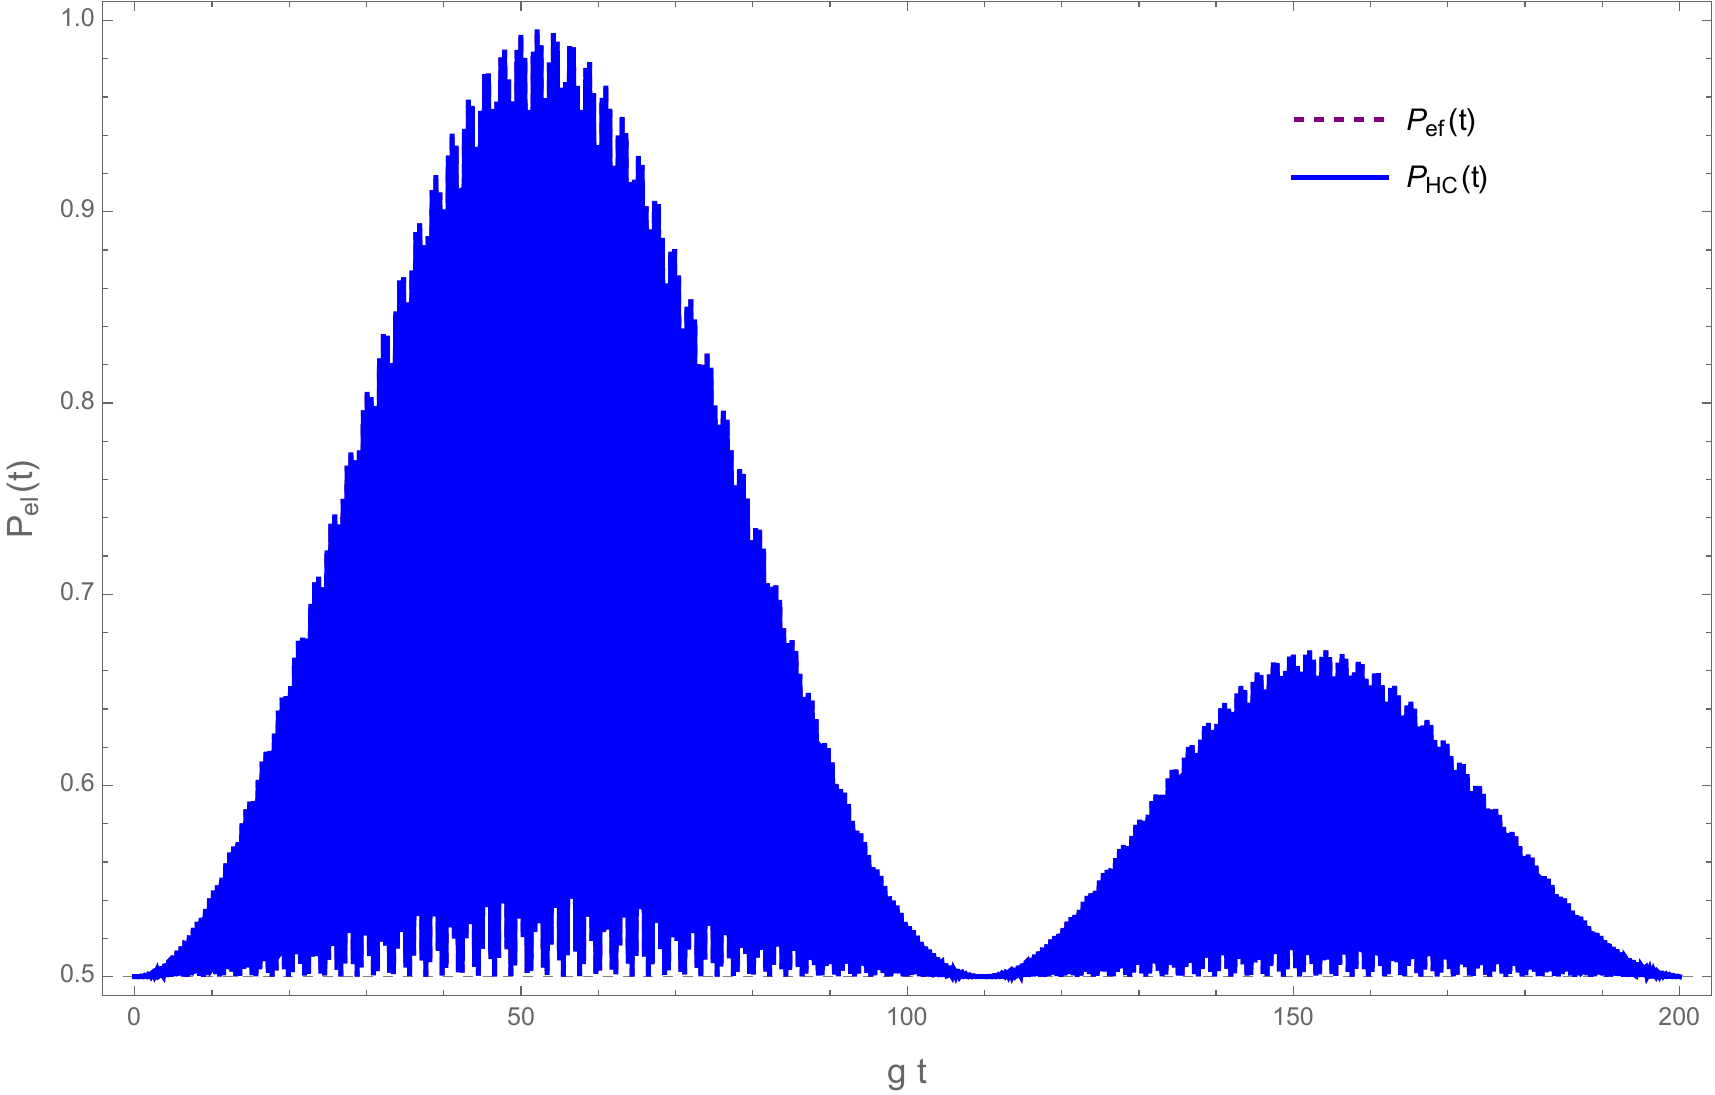
\includegraphics[width=0.88\textwidth]{../../notas-doctorado/imgs/Entrelazamiento/pureza-fonon-coherente-polariton.png}
  \caption{Pureza electr\'onica para un estado coherente fon\'onico dentro de
  un bloque polarit\'onico. Las evoluciones obtenidas con el hamiltoniano
  efectivo y con el hamiltoniano completo de Holstein--Cummings son
  pr\'acticamente id\'enticas. Los m\'aximos $P_{\mathrm{el}}=1$ identifican
  instantes en los que la bipartici\'on electr\'on frente a fot\'on--fon\'on es
  separable.}
\end{figure}

El estado evolucionado dentro de un bloque $n$ fijo se escribe como
\begin{equation}
\begin{aligned}
  \ket{\tilde\Psi_n(t)}
  ={}&
  p_{n0}^{-}(t)\ket{-,n,0}
  \\
  &+
  \sum_{m=1}^{\infty}
  \left[
  p_{nm}^{+}(t)\ket{+,n,m-1}
  +
  p_{nm}^{-}(t)\ket{-,n,m}
  \right].
\end{aligned}
\end{equation}
Recordando la definici\'on de los polaritones,
\begin{equation}
  \ket{\pm,n}
  =
  \frac{1}{\sqrt2}
  \left(
  \ket{e,n-1}\pm\ket{g,n}
  \right),
\end{equation}
el estado puede reagruparse de acuerdo con sus dos ramas electr\'onicas:
\begin{equation}
  \ket{\tilde\Psi_n(t)}
  =
  \ket{\chi_e(t)}\ket e
  +
  \ket{\chi_g(t)}\ket g,
\end{equation}
donde
\begin{equation}
  \ket{\chi_e(t)}
  =
  \frac{\ket{n-1}}{\sqrt2}
  \sum_{k=0}^{\infty}
  \left[
  p_{n,k+1}^{+}(t)+p_{nk}^{-}(t)
  \right]\ket k,
\end{equation}
\begin{equation}
  \ket{\chi_g(t)}
  =
  \frac{\ket n}{\sqrt2}
  \sum_{k=0}^{\infty}
  \left[
  p_{n,k+1}^{+}(t)-p_{nk}^{-}(t)
  \right]\ket k.
\end{equation}
Separando expl\'icitamente la parte fot\'onica de la vibracional se obtiene
\begin{equation}
  \ket{\tilde\Psi_n(t)}
  =
  \ket e\ket{n-1}\ket{\phi_e(t)}
  +
  \ket g\ket n\ket{\phi_g(t)},
\end{equation}
con
\begin{equation}
  \boxed{
  \ket{\phi_e(t)}
  =
  \frac{1}{\sqrt2}
  \sum_{k=0}^{\infty}
  \left[
  p_{n,k+1}^{+}(t)+p_{nk}^{-}(t)
  \right]\ket k,
  }
\end{equation}
\begin{equation}
  \boxed{
  \ket{\phi_g(t)}
  =
  \frac{1}{\sqrt2}
  \sum_{k=0}^{\infty}
  \left[
  p_{n,k+1}^{+}(t)-p_{nk}^{-}(t)
  \right]\ket k.
  }
\end{equation}

Las dos ramas contienen los estados fot\'onicos ortogonales $\ket{n-1}$ y
$\ket n$. Por esta raz\'on la matriz de densidad electr\'onica reducida es
siempre diagonal:
\begin{equation}
  \hat\rho_{\mathrm{el}}(t)
  =
  P_e(t)\ket e\bra e
  +
  P_g(t)\ket g\bra g,
\end{equation}
donde
\begin{equation}
  P_e(t)=\braket{\phi_e(t)|\phi_e(t)},
  \qquad
  P_g(t)=\braket{\phi_g(t)|\phi_g(t)},
  \qquad
  P_e(t)+P_g(t)=1.
\end{equation}
Definiendo la inversi\'on electr\'onica como
\begin{equation}
  W(t)=P_e(t)-P_g(t),
\end{equation}
se tiene
\begin{equation}
  P_e(t)=\frac{1+W(t)}{2},
  \qquad
  P_g(t)=\frac{1-W(t)}{2},
\end{equation}
y la pureza queda
\begin{equation}
  \boxed{
  P_{\mathrm{el}}(t)
  =
  P_e^2(t)+P_g^2(t)
  =
  \frac{1+W^2(t)}{2}.
  }
\end{equation}

Para que la bipartici\'on sea separable en un tiempo $t_*$ se impone
\begin{equation}
  P_{\mathrm{el}}(t_*)=1
  \quad\Longrightarrow\quad
  |W(t_*)|=1.
\end{equation}
Como $P_e+P_g=1$, una pureza unitaria solo puede ocurrir de dos maneras:
\begin{equation}
  (P_e,P_g)=(1,0)
  \qquad\text{o}\qquad
  (P_e,P_g)=(0,1).
\end{equation}
Si $W(t_*)=1$, entonces $\ket{\phi_g(t_*)}=0$ y el estado completo se reduce a
\begin{equation}
  \boxed{
  \ket{\tilde\Psi_n(t_*)}
  =
  \ket e\otimes\ket{n-1}\otimes\ket{\phi_e(t_*)}.
  }
\end{equation}
Si $W(t_*)=-1$, entonces $\ket{\phi_e(t_*)}=0$ y queda
\begin{equation}
  \boxed{
  \ket{\tilde\Psi_n(t_*)}
  =
  \ket g\otimes\ket n\otimes\ket{\phi_g(t_*)}.
  }
\end{equation}
En ambos casos el estado es producto respecto de los tres subsistemas:
electr\'on, cavidad y vibraci\'on.

Para obtener el estado electr\'onico excitado debe cumplirse
\begin{equation}
  \ket{\phi_g(t_*)}
  =
  \frac{1}{\sqrt2}
  \sum_{k=0}^{\infty}
  \left[
  p_{n,k+1}^{+}(t_*)-p_{nk}^{-}(t_*)
  \right]\ket k
  =0.
\end{equation}
La independencia lineal de los estados de Fock exige, para cada $k$,
\begin{equation}
  p_{n,k+1}^{+}(t_*)=p_{nk}^{-}(t_*).
\end{equation}
Por tanto,
\begin{equation}
  \ket{\phi_e(t_*)}
  =
  \sqrt2
  \sum_{k=0}^{\infty}p_{nk}^{-}(t_*)\ket k.
\end{equation}
De manera an\'aloga, cuando se alcanza la rama electr\'onica base,
\begin{equation}
  \ket{\phi_g(t_*)}
  =
  -\sqrt2
  \sum_{k=0}^{\infty}p_{nk}^{-}(t_*)\ket k.
\end{equation}
La inversi\'on determina cu\'al de estos dos estados producto se alcanza para
una preparaci\'on inicial dada. Despu\'es es necesario reconstruir las
amplitudes $p_{nm}^{\pm}(t_*)$ para conocer el estado vibracional concreto.

En resonancia, $\delta_n=0$, la inversi\'on electr\'onica para un estado
coherente fon\'onico dentro de un bloque polarit\'onico es
\begin{equation}
  \boxed{
  W(t)
  =
  2\sin(2\nu t)
  \sum_{m=0}^{\infty}
  \tilde c_{m+1}\tilde c_m
  \sin\left(\frac{\kappa_{m+1}t}{2}\right)
  \cos\left(\frac{\kappa_mt}{2}\right),
  \qquad
  \kappa_m=\nu\lambda\sqrt m.
  }
\end{equation}
Esta expresi\'on permite localizar los instantes $t_*$ mediante la condici\'on
$W(t_*)=\pm1$.

\section{Estado separable inicial para generar un GHZ}

Los estados GHZ obtenidos al evolucionar dentro de un solo doblete parten de
un polarit\'on, que ya est\'a entrelazado en los grados electr\'onico y
fot\'onico. Para generar un GHZ a partir de un estado completamente separable
se necesita salir de un doblete aislado. Se propone entonces el estado inicial
\begin{equation}
  \boxed{
  \ket{\tilde\Psi(0)}
  =
  \ket e\otimes\ket{n-1}
  \otimes
  \left(
  \cos\theta\ket m
  +e^{\ii\phi}\sin\theta\ket{m+1}
  \right).
  }
\end{equation}
Este estado es separable respecto de los tres subsistemas. Para abreviar se
definen
\begin{equation}
  a=\cos\theta,
  \qquad
  b=e^{\ii\phi}\sin\theta.
\end{equation}
Usando
\begin{equation}
  \ket{e,n-1}
  =
  \frac{\ket{+,n}+\ket{-,n}}{\sqrt2},
\end{equation}
el estado inicial se convierte en
\begin{equation}
\begin{aligned}
  \ket{\tilde\Psi(0)}
  &=\frac{1}{\sqrt2}
  \left(\ket{+,n}+\ket{-,n}\right)
  \otimes
  \left(a\ket m+b\ket{m+1}\right)
  \\
  &=
  \frac{1}{\sqrt2}
  \left[
  a\ket{+,n,m}
  +a\ket{-,n,m}
  +b\ket{+,n,m+1}
  +b\ket{-,n,m+1}
  \right].
\end{aligned}
\end{equation}

El hamiltoniano efectivo acopla
\begin{equation}
  \ket{+,n,r-1}
  \longleftrightarrow
  \ket{-,n,r}.
\end{equation}
Por ello, los cuatro t\'erminos de la preparaci\'on inicial se distribuyen en
tres dobletes distintos:
\begin{equation}
  \boxed{
  \begin{gathered}
  \ket{+,n,m}\longleftrightarrow\ket{-,n,m+1},
  \\
  \ket{+,n,m-1}\longleftrightarrow\ket{-,n,m},
  \\
  \ket{+,n,m+1}\longleftrightarrow\ket{-,n,m+2}.
  \end{gathered}
  }
\end{equation}
Esta participaci\'on simult\'anea de tres dobletes es el ingrediente que permite
partir de un producto y construir posteriormente correlaciones tripartitas.

\section{Evoluci\'on resonante en los tres dobletes}

En resonancia,
\begin{equation}
  \delta_n=0,
  \qquad
  \Omega_{nr}^{\mathrm{ef}}=\kappa_r,
\end{equation}
el operador de evoluci\'on del doblete $r$ es
\begin{equation}
  \boxed{
  \hat U_{nr}(t)
  =
  e^{-\ii A_{nr}t}
  \left[
  \cos\left(\frac{\kappa_rt}{2}\right)\Id
  +
  \ii\sin\left(\frac{\kappa_rt}{2}\right)\hat\sigma_x
  \right].
  }
\end{equation}
Aqu\'i, $\hat\sigma_x$ es el operador de intercambio restringido al doblete
$\{\ket{+,n,r-1},\ket{-,n,r}\}$:
\begin{equation}
  \hat\sigma_x
  =
  \ket{+,n,r-1}\bra{-,n,r}
  +
  \ket{-,n,r}\bra{+,n,r-1}.
\end{equation}
Se introducen las abreviaturas
\begin{equation}
  C_r=\cos\left(\frac{\kappa_rt}{2}\right),
  \qquad
  S_r=\sin\left(\frac{\kappa_rt}{2}\right).
\end{equation}
Las dos evoluciones elementales son
\begin{equation}
  \ket{+,n,r-1}
  \longrightarrow
  e^{-\ii A_{nr}t}
  \left[
  C_r\ket{+,n,r-1}
  +\ii S_r\ket{-,n,r}
  \right],
\end{equation}
\begin{equation}
  \ket{-,n,r}
  \longrightarrow
  e^{-\ii A_{nr}t}
  \left[
  C_r\ket{-,n,r}
  +\ii S_r\ket{+,n,r-1}
  \right].
\end{equation}
Aplic\'andolas a cada t\'ermino del estado inicial,
\begin{equation}
  \ket{+,n,m}
  \longrightarrow
  e^{-\ii A_{n,m+1}t}
  \left[
  C_{m+1}\ket{+,n,m}
  +\ii S_{m+1}\ket{-,n,m+1}
  \right],
\end{equation}
\begin{equation}
  \ket{-,n,m}
  \longrightarrow
  e^{-\ii A_{nm}t}
  \left[
  C_m\ket{-,n,m}
  +\ii S_m\ket{+,n,m-1}
  \right],
\end{equation}
\begin{equation}
  \ket{+,n,m+1}
  \longrightarrow
  e^{-\ii A_{n,m+2}t}
  \left[
  C_{m+2}\ket{+,n,m+1}
  +\ii S_{m+2}\ket{-,n,m+2}
  \right],
\end{equation}
\begin{equation}
  \ket{-,n,m+1}
  \longrightarrow
  e^{-\ii A_{n,m+1}t}
  \left[
  C_{m+1}\ket{-,n,m+1}
  +\ii S_{m+1}\ket{+,n,m}
  \right].
\end{equation}

La evoluci\'on completa queda
\begin{equation}
\begin{aligned}
  \ket{\tilde\Psi(t)}
  =\frac{1}{\sqrt2}\Big\{&
  a e^{-\ii A_{n,m+1}t}
  \left[
  C_{m+1}\ket{+,n,m}
  +\ii S_{m+1}\ket{-,n,m+1}
  \right]
  \\
  &+
  a e^{-\ii A_{nm}t}
  \left[
  C_m\ket{-,n,m}
  +\ii S_m\ket{+,n,m-1}
  \right]
  \\
  &+
  b e^{-\ii A_{n,m+2}t}
  \left[
  C_{m+2}\ket{+,n,m+1}
  +\ii S_{m+2}\ket{-,n,m+2}
  \right]
  \\
  &+
  b e^{-\ii A_{n,m+1}t}
  \left[
  C_{m+1}\ket{-,n,m+1}
  +\ii S_{m+1}\ket{+,n,m}
  \right]
  \Big\}.
\end{aligned}
\end{equation}

Factorizando las ramas $\ket{+,n}$ y $\ket{-,n}$ se obtiene
\begin{equation}
  \boxed{
  \ket{\tilde\Psi(t)}
  =
  \ket{+,n}\ket{\Phi_+(t)}
  +
  \ket{-,n}\ket{\Phi_-(t)}.
  }
\end{equation}
Los dos estados vibracionales son
\begin{equation}
\begin{aligned}
  \ket{\Phi_+(t)}
  =\frac{1}{\sqrt2}\Big[&
  \ii a e^{-\ii A_{nm}t}S_m\ket{m-1}
  \\
  &+
  e^{-\ii A_{n,m+1}t}
  \left(aC_{m+1}+\ii bS_{m+1}\right)\ket m
  \\
  &+
  b e^{-\ii A_{n,m+2}t}C_{m+2}\ket{m+1}
  \Big],
\end{aligned}
\end{equation}
\begin{equation}
\begin{aligned}
  \ket{\Phi_-(t)}
  =\frac{1}{\sqrt2}\Big[&
  a e^{-\ii A_{nm}t}C_m\ket m
  \\
  &+
  e^{-\ii A_{n,m+1}t}
  \left(\ii aS_{m+1}+bC_{m+1}\right)\ket{m+1}
  \\
  &+
  \ii b e^{-\ii A_{n,m+2}t}S_{m+2}\ket{m+2}
  \Big].
\end{aligned}
\end{equation}

La energ\'ia com\'un del doblete depende linealmente de $r$:
\begin{equation}
  A_{nr}
  =
  n\Omega+\frac{\nu\lambda^2}{4}
  +\nu\left(r-\frac12\right)
  =
  A_n^{(0)}+\nu r,
\end{equation}
\begin{equation}
  A_n^{(0)}
  =
  n\Omega+\frac{\nu\lambda^2}{4}-\frac{\nu}{2}.
\end{equation}
Por tanto,
\begin{equation}
  e^{-\ii A_{nr}t}
  =
  e^{-\ii A_n^{(0)}t}e^{-\ii r\nu t}.
\end{equation}
El primer factor es com\'un a todo el estado y representa una fase global, que
puede descartarse. Definiendo el tiempo adimensional
\begin{equation}
  \tau=\nu t,
\end{equation}
los estados vibracionales toman la forma
\begin{equation}
  \boxed{
  \begin{aligned}
  \ket{\Phi_+(t)}
  =\frac{1}{\sqrt2}\Big[&
  \ii a e^{-\ii m\tau}S_m\ket{m-1}
  \\
  &+e^{-\ii(m+1)\tau}
  \left(aC_{m+1}+\ii bS_{m+1}\right)\ket m
  \\
  &+b e^{-\ii(m+2)\tau}C_{m+2}\ket{m+1}
  \Big],
  \end{aligned}
  }
\end{equation}
\begin{equation}
  \boxed{
  \begin{aligned}
  \ket{\Phi_-(t)}
  =\frac{1}{\sqrt2}\Big[&
  a e^{-\ii m\tau}C_m\ket m
  \\
  &+e^{-\ii(m+1)\tau}
  \left(\ii aS_{m+1}+bC_{m+1}\right)\ket{m+1}
  \\
  &+\ii b e^{-\ii(m+2)\tau}S_{m+2}\ket{m+2}
  \Big].
  \end{aligned}
  }
\end{equation}

\section{Condiciones para obtener un estado GHZ}

Se regresa a la base opto-electr\'onica mediante
\begin{equation}
  \ket{\pm,n}
  =
  \frac{\ket e\ket{n-1}\pm\ket g\ket n}{\sqrt2}.
\end{equation}
Entonces,
\begin{equation}
\begin{aligned}
  \ket{\tilde\Psi(t)}
  ={}&
  \ket e\ket{n-1}
  \frac{\ket{\Phi_+(t)}+\ket{\Phi_-(t)}}{\sqrt2}
  \\
  &+
  \ket g\ket n
  \frac{\ket{\Phi_+(t)}-\ket{\Phi_-(t)}}{\sqrt2}.
\end{aligned}
\end{equation}
Definiendo
\begin{equation}
  \ket{\chi_e(t)}
  =
  \frac{\ket{\Phi_+(t)}+\ket{\Phi_-(t)}}{\sqrt2},
  \qquad
  \ket{\chi_g(t)}
  =
  \frac{\ket{\Phi_+(t)}-\ket{\Phi_-(t)}}{\sqrt2},
\end{equation}
se obtiene
\begin{equation}
  \ket{\tilde\Psi(t)}
  =
  \ket e\ket{n-1}\ket{\chi_e(t)}
  +
  \ket g\ket n\ket{\chi_g(t)}.
\end{equation}

Para que este estado sea un GHZ tripartito m\'aximamente entrelazado se
requiere que las ramas electr\'onicas tengan el mismo peso y que sus estados
vibracionales sean ortogonales:
\begin{equation}
  \|\chi_e(t_*)\|^2
  =
  \|\chi_g(t_*)\|^2
  =
  \frac12,
  \qquad
  \braket{\chi_g(t_*)|\chi_e(t_*)}=0.
\end{equation}
Las normas son
\begin{equation}
\begin{aligned}
  \braket{\chi_e|\chi_e}
  &={}
  \frac12
  \left[
  \braket{\Phi_+|\Phi_+}
  +\braket{\Phi_+|\Phi_-}
  +\braket{\Phi_-|\Phi_+}
  +\braket{\Phi_-|\Phi_-}
  \right]
  \\
  &=
  \frac12+\operatorname{Re}\braket{\Phi_+|\Phi_-},
\end{aligned}
\end{equation}
\begin{equation}
  \braket{\chi_g|\chi_g}
  =
  \frac12-\operatorname{Re}\braket{\Phi_+|\Phi_-}.
\end{equation}
La igualdad de pesos exige
\begin{equation}
  \operatorname{Re}\braket{\Phi_+(t_*)|\Phi_-(t_*)}=0.
\end{equation}
Por otra parte,
\begin{equation}
\begin{aligned}
  \braket{\chi_g|\chi_e}
  ={}&
  \frac12
  \left[
  \braket{\Phi_+|\Phi_+}
  -\braket{\Phi_+|\Phi_-}
  +\braket{\Phi_-|\Phi_+}
  -\braket{\Phi_-|\Phi_-}
  \right]
  \\
  ={}&
  \frac12
  \left(
  \braket{\Phi_+|\Phi_+}
  -\braket{\Phi_-|\Phi_-}
  \right)
  -\ii\operatorname{Im}\braket{\Phi_+|\Phi_-}.
\end{aligned}
\end{equation}
Por tanto, la ortogonalidad requiere simult\'aneamente
\begin{equation}
  \braket{\Phi_+|\Phi_+}
  =
  \braket{\Phi_-|\Phi_-},
  \qquad
  \operatorname{Im}\braket{\Phi_+|\Phi_-}=0.
\end{equation}
Como
\begin{equation}
  \braket{\Phi_+|\Phi_+}
  +
  \braket{\Phi_-|\Phi_-}=1,
\end{equation}
las condiciones completas pueden escribirse de manera compacta como
\begin{equation}
  \boxed{
  \|\Phi_+(t_*)\|^2
  =
  \|\Phi_-(t_*)\|^2
  =
  \frac12,
  \qquad
  \braket{\Phi_+(t_*)|\Phi_-(t_*)}=0.
  }
\end{equation}

\section{Primera condici\'on: igualdad de normas}

Se calcula la diferencia entre las normas:
\begin{equation}
\begin{aligned}
  \|\Phi_+\|^2-\|\Phi_-\|^2
  =\frac12\Big[&
  |a|^2S_m^2
  +(aC_{m+1}-\ii b^*S_{m+1})
   (aC_{m+1}+\ii bS_{m+1})
  +|b|^2C_{m+2}^2
  \\
  &-|a|^2C_m^2
  -(-\ii aS_{m+1}+b^*C_{m+1})
   (\ii aS_{m+1}+bC_{m+1})
  -|b|^2S_{m+2}^2
  \Big].
\end{aligned}
\end{equation}
Los dos productos no triviales son
\begin{equation}
\begin{aligned}
  &(aC_{m+1}-\ii b^*S_{m+1})
   (aC_{m+1}+\ii bS_{m+1})
  \\
  &\qquad=
  a^2C_{m+1}^2
  +|b|^2S_{m+1}^2
  -2a\operatorname{Im}(b)C_{m+1}S_{m+1},
\end{aligned}
\end{equation}
\begin{equation}
\begin{aligned}
  &(-\ii aS_{m+1}+b^*C_{m+1})
   (\ii aS_{m+1}+bC_{m+1})
  \\
  &\qquad=
  a^2S_{m+1}^2
  +|b|^2C_{m+1}^2
  +2a\operatorname{Im}(b)C_{m+1}S_{m+1}.
\end{aligned}
\end{equation}
Sustituyendo ambos resultados,
\begin{equation}
\begin{aligned}
  \|\Phi_+\|^2-\|\Phi_-\|^2
  =\frac12\Big[&
  a^2(S_m^2-C_m^2)
  +(a^2-|b|^2)(C_{m+1}^2-S_{m+1}^2)
  \\
  &+|b|^2(C_{m+2}^2-S_{m+2}^2)
  -4a\operatorname{Im}(b)C_{m+1}S_{m+1}
  \Big].
\end{aligned}
\end{equation}
Con
\begin{equation}
  a=\cos\theta,
  \qquad
  |b|^2=\sin^2\theta,
  \qquad
  \operatorname{Im}(b)=\sin\phi\sin\theta,
\end{equation}
se obtiene
\begin{equation}
\begin{aligned}
  \|\Phi_+\|^2-\|\Phi_-\|^2
  =\frac12\Big[&
  \cos^2\theta(S_m^2-C_m^2)
  +\cos(2\theta)(C_{m+1}^2-S_{m+1}^2)
  \\
  &+\sin^2\theta(C_{m+2}^2-S_{m+2}^2)
  -4\cos\theta\sin\theta\sin\phi\,
  C_{m+1}S_{m+1}
  \Big].
\end{aligned}
\end{equation}
Ahora se define
\begin{equation}
  x_r=\frac{\lambda\sqrt r\,\tau}{2},
  \qquad
  C_r=\cos x_r,
  \qquad
  S_r=\sin x_r.
\end{equation}
Usando
\begin{equation}
  \cos^2x-\sin^2x=\cos(2x),
  \qquad
  2\sin x\cos x=\sin(2x),
\end{equation}
la condici\'on $\|\Phi_+\|^2-\|\Phi_-\|^2=0$ se transforma en
\begin{equation}
  \boxed{
  \begin{aligned}
  F_1(\theta,\tau)
  ={}&
  -\cos^2\theta\cos(\lambda\sqrt m\,\tau)
  +\cos(2\theta)\cos(\lambda\sqrt{m+1}\,\tau)
  \\
  &+\sin^2\theta\cos(\lambda\sqrt{m+2}\,\tau)
  -\sin\phi\sin(2\theta)
  \sin(\lambda\sqrt{m+1}\,\tau)
  =0.
  \end{aligned}
  }
\end{equation}

\section{Segunda condici\'on: ortogonalidad}

Debido al soporte de $\ket{\Phi_+}$ y $\ket{\Phi_-}$ en la base de Fock,
solo los estados $\ket m$ y $\ket{m+1}$ contribuyen a su producto interno.
El c\'alculo da
\begin{equation}
\begin{aligned}
  \braket{\Phi_+(t)|\Phi_-(t)}
  =\frac12\Big[&
  a e^{-\ii m\tau}C_m
  e^{\ii(m+1)\tau}
  (aC_{m+1}-\ii b^*S_{m+1})
  \\
  &+
  b^* e^{\ii(m+2)\tau}C_{m+2}
  e^{-\ii(m+1)\tau}
  (\ii aS_{m+1}+bC_{m+1})
  \Big]
  \\
  =\frac{e^{\ii\tau}}{2}\Big[&
  C_{m+1}(a^2C_m+|b|^2C_{m+2})
  +\ii ab^*S_{m+1}(-C_m+C_{m+2})
  \Big].
\end{aligned}
\end{equation}
Al sustituir $a=\cos\theta$ y $b=e^{\ii\phi}\sin\theta$, y usar
\begin{equation}
  \ii e^{-\ii\phi}=\sin\phi+\ii\cos\phi,
\end{equation}
las partes real e imaginaria del factor entre corchetes deben anularse:
\begin{equation}
\begin{aligned}
  &C_{m+1}
  \left(
  \cos^2\theta\,C_m
  +\sin^2\theta\,C_{m+2}
  \right)
  \\
  &\qquad+
  \frac12\sin(2\theta)\sin\phi\,
  S_{m+1}(C_{m+2}-C_m)=0,
\end{aligned}
\end{equation}
\begin{equation}
  \frac12\sin(2\theta)\cos\phi\,
  S_{m+1}(-C_m+C_{m+2})=0.
\end{equation}
Se elige
\begin{equation}
  \phi=\frac{\pi}{2}.
\end{equation}
Con esta elecci\'on la segunda ecuaci\'on se anula autom\'aticamente y la
primera queda
\begin{equation}
\begin{aligned}
  &C_{m+1}
  \left(
  \cos^2\theta\,C_m
  +\sin^2\theta\,C_{m+2}
  \right)
  \\
  &\qquad-
  \frac12\sin(2\theta)S_{m+1}(C_m-C_{m+2})=0.
\end{aligned}
\end{equation}
Sustituyendo las definiciones de $C_r$ y $S_r$ se obtiene la segunda
ecuaci\'on trascendente:
\begin{equation}
  \boxed{
  \begin{aligned}
  F_2(\theta,\tau)
  ={}&
  \cos\left(\frac{\lambda\sqrt{m+1}\,\tau}{2}\right)
  \Bigg[
  \cos^2\theta
  \cos\left(\frac{\lambda\sqrt m\,\tau}{2}\right)
  \\
  &\qquad+
  \sin^2\theta
  \cos\left(\frac{\lambda\sqrt{m+2}\,\tau}{2}\right)
  \Bigg]
  \\
  &-
  \frac12\sin(2\theta)
  \sin\left(\frac{\lambda\sqrt{m+1}\,\tau}{2}\right)
  \Bigg[
  \cos\left(\frac{\lambda\sqrt m\,\tau}{2}\right)
  \\
  &\qquad-
  \cos\left(\frac{\lambda\sqrt{m+2}\,\tau}{2}\right)
  \Bigg]
  =0.
  \end{aligned}
  }
\end{equation}

\section{Soluci\'on simult\'anea y protocolo final}

Para $\phi=\pi/2$, los valores de $\theta$ y $\tau$ deben satisfacer
simult\'aneamente
\begin{equation}
  \boxed{
  F_1(\theta,\tau)=0,
  \qquad
  F_2(\theta,\tau)=0.
  }
\end{equation}
La b\'usqueda num\'erica presentada en el manuscrito produce la ra\'iz
\begin{equation}
  \boxed{
  \theta_*=0.548014622536,
  \qquad
  \tau_*=20.1362696530.
  }
\end{equation}
En consecuencia, la preparaci\'on vibracional separable que debe acompa\~nar a
$\ket e\ket{n-1}$ es
\begin{equation}
  \boxed{
  \ket{\psi_{\mathrm{vib}}(0)}
  =
  \cos\theta_*\ket m
  +\ii\sin\theta_*\ket{m+1}.
  }
\end{equation}
Tras evolucionar resonantemente durante el tiempo
\begin{equation}
  t_*=\frac{\tau_*}{\nu},
\end{equation}
las dos ramas electr\'onico--fot\'onicas tienen igual probabilidad y los
estados vibracionales que las acompa\~nan son ortogonales. Por tanto,
\begin{equation}
  \ket{\tilde\Psi(t_*)}
  =
  \ket e\ket{n-1}\ket{\chi_e(t_*)}
  +
  \ket g\ket n\ket{\chi_g(t_*)},
\end{equation}
con
\begin{equation}
  \|\chi_e(t_*)\|^2
  =
  \|\chi_g(t_*)\|^2
  =
  \frac12,
  \qquad
  \braket{\chi_g(t_*)|\chi_e(t_*)}=0.
\end{equation}
Estas son precisamente las condiciones de un estado GHZ tripartito, salvo
fases y elecciones locales de la base l\'ogica. El protocolo genera as\'i
entrelazamiento genuinamente tripartito a partir de una preparaci\'on inicial
completamente separable.

\end{document}
